\chapter{Literature Review}\label{ch:LitReview}

The theory behind GPS tracking loops has intellectual roots in classical control theory. Ultimately a \ac{GNSS} tracking loop is a control system, attempting to generate a local replica of an incoming signal, with minimal error. Nise \cite{Nise} provides a thorough overview of control theory, while Gardner \cite{Gardner} provides an excellent overview of the operation of PLL, from the viewpoint of classical control theory.  

More recently however, GNSS receiver tracking loop design has evolved in order to meet new challenges, in particular high dynamics and weak signal strength. While high dynamics and weak signal strength may initially appear to be disparate concepts, they are intricately linked through the bandwidth time product($B_LT$). 

The designer of a tracking loop has three different attributes that they can adjust to meet the desired performance 
\begin{enumerate}
\item{Loop architecture}
\item{Loop order}
\item{Loop coefficients}
\end{enumerate}

Of these, the most effort has been expended on determining the optimum loop coefficients. 

\section{Loop architecture}

The choice of architecture strongly determines the overall performance of a \ac{GNSS} receiver, in particular, the architecture must be decided upon with the application of the receiver in mind. To quote Kaplan: 
\begin{quotation}
"There is a paradox that the GPS receiver designer must solve in the design of the pre-detection integration time and the discriminator and loop filter functions of the carrier tracking loop. To tolerate dynamic stress, the pre-detection integration time should be short, the discriminator should be an \ac{FLL}, and the carrier loop filter bandwidth should be wide.

However, for the carrier measurements to be accurate (have low noise), the pre-detection integration time should be long, the discriminator should be a \ac{PLL}, and the carrier loop filter noise bandwidth should be narrow. In practice, some compromise must be made to resolve this paradox."\cite{Kaplan}
\end{quotation}

Ward performs a sophisticated analysis of the trade-off between a \ac{PLL} and a \ac{FLL}, stating that 
\begin{quotation}
"A well-designed frequency lock loop (FLL) will outperform
a well-designed phase lock loop (PLL) tracking threshold
under dynamic stress and RF interference (RFI) conditions.
However, the PLL will significantly outperform the FLL
measurement accuracy."\cite{ward1998}
\end{quotation}

In \cite{ward1998}, an innovative carrier tracking loop design technique which
integrates both the FLL and the PLL characteristics, called an FLL-assisted-PLL is developed. This is the architecture, which can be seen in figure \ref{fig:Architecture} is used in the Namuru receiver, and is further described by Ward in \cite{Kaplan}.

\begin{figure}[!htb] 
    \centering
    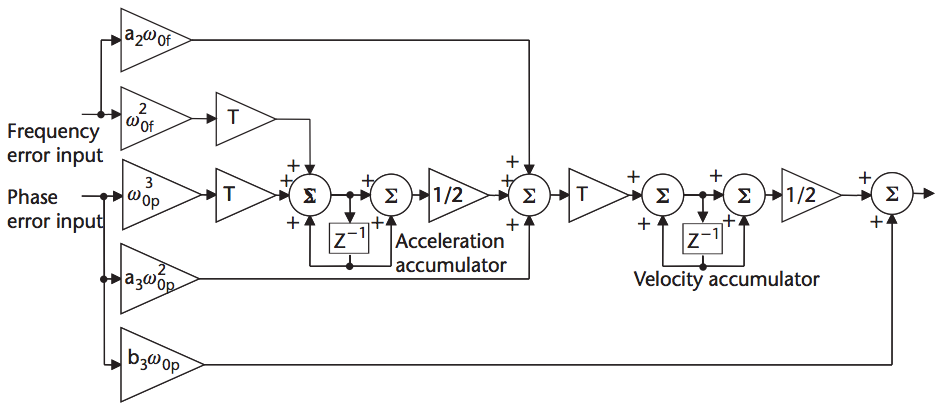
\includegraphics[width=1\textwidth]{Architecture.png} 
    \caption{The discrete implementation of the Ward architecture (FLL-assisted-PLL). Note that the integrators have been implemented using the bilinear transform \cite{Ward}.}
    \label{fig:Architecture}
\end{figure}

\section{Loop order}
From a careful analysis of control theory, we can gain an understanding of the importance of the loop order on the performance on a tracking loop. Kazemi \cite{KazemiPHD,Kazemi2008} and Gardner \cite{Gardner} both spend a significant amount of time covering the development of a Laplace domain model of a \ac{PLL}. 

Ultimately, a trade-off exists between filter order and stability. First and second order filter are unconditionally stable in the Laplace domain, however they are not as effective as third order loops at coping with dynamics. For example, the residual error of a second order loop is acceleration. This makes it unsuitable for any application where sustained acceleration is likely to be encountered, as the error will increase over time, until phase lock is lost. In most real world scenarios, sustained acceleration is limited, due to limits on maximum achievable velocities. For space based applications however, velocities of thousands of meters per second are routinely achieved. Hence while a second order loop may be suitable for terrestrial applications, a third order loops is required for spaced based applications. 

\begin{table}[h]
\centering
\begin{tabular}{|l|l|l|l|}
\hline
Loop order & Filter order & Residual Error & Stability                               \\ \hline
1          & 0            & Velocity       & Stable                                  \\ \hline
2          & 1            & Acceleration   & Stable                                  \\ \hline
3          & 2            & Jerk           & Remains stable at $B_n$ \textless 18 Hz \\ \hline
\end{tabular}
\caption{Loop order behavior}
\label{table:LoopOrders}
\end{table}

\section{Loop coefficients}

The selection of suitable loop coefficients is the aspect of \ac{PLL} design that has received the most attention in the literature. A number of competing approaches exist, and the state of the art has evolved over time, as \ac{GPS} is applied to new and more challenging applications, in particular high dynamics and weak signal applications.

\subsection{Design in Laplace domain, convert to Z Domain}
A popular method for designing a \ac{DPLL} is to design a \ac{PLL} in the Laplace domain, and then convert it to a \ac{DPLL} using a transform. Examples of analog to digital transformation methods include the bilinear, boxcar and impulse invariant transforms. This method is very common as it results in an a set of easy to follow design equations, which produce tracking loops which are suitable for general use. In the literature, this approach is used by Spilker\cite{Spilker}, Gardner\cite{Gardner}, Kaplan\cite{Kaplan} and Ward\cite{Ward}. In particular, the Ward method of determining loop co-efficients is the one used in the design of the Namuru receiver.

A key advantage of this method is that analysis of the loops can be carried out in the Laplace domain, using tools from classical control theory, for example root locus\cite{Nise}. This is useful, because it provides an understanding of how the stability of the system evolves with changing parameters. 

One of the disadvantages of this procedure, is that the use of a transformation from the Laplace domain to the Z domain results in a filter that is an approximation of the filter in the Laplace domain. If the integration time is sufficiently large, and conversely, the sampling frequency is sufficiently small, then the stability of the filter can be compromised. 

A figure of merit that is useful in comparing the \ac{PLL} designed by a particular method is the product between loop noise bandwidth and integration time ($B_LT$). The concept of the $B_LT$ further re-enforces the ultimate trade-off between integration time (sensitivity) and loop noise bandwidth (dynamics). The maximum stable $B_LT$ achievable by designing in the Laplace domain is approximately 0.4 \cite{Kazemi2008,KazemiPHD}

Finally, it is also important to consider that analogue analysis has made linearizing assumptions, and transferring analogue analysis to the digital domain is also non-linear and approximate\cite{Dempster}. 

\subsection{Design by minimizing the loop phase jitter}

Kazemi\cite{KazemiPHD,Kazemi2008} provides the most sophisticated analysis of \ac{PLL}. In particular, Kazemi takes into account the effect of averaging and delay, introduced by the integration and dump, allowing stable tracking loops to be developed with large $B_LT$. While Kazemi focuses on the development of receivers for weak signal tracking, his work is still applicable to high dynamics, as increasing the integration time of a receiver for a given noise band with, is equivalent to increasing the noise bandwidth, for a given integration time. 

While the methods described by Kazemi is highly complex, it theoretically offers an order of magnitude improvement in achievable $B_LT$. Kazemi also describes a detailed test plan, for evaluating the performance of the tracking loops, both on real-world and simulated signals, which is very instructive for critically evaluating the performance of new algorithms.
















